\section{Stäbe}
In dieser Versuchsreihe wurde das Elastizitätsmodul von vier verschiedenen Stäben bestimmt.
\subsection{Methoden}
Die Durchführung dieses Experimentes erfolgte in zwei Abschnitten.
Im ersten Abschnitt wurde die Länge und die Dicke von vier verschiedenen Stäben bestimmt.
Die Dicke der Stäbe wurde mit einer Mikrometerschraube gemessen und die Länge mit einem Maßband, wobei hier von einem enden des Stabes bis zu Aufhängepunkt des Gewichtes gemessen wurde.
Da die Dicke der Stäbe mit einer Potenz von vier in das Elastizitätsmodul eingeht wurde sie an fünf stellen drei mal bestimmt.  Nach Abschluss dieser Messungen wurde im zweiten Abschnitt die Durchbiegung der Materialien in Abhängigkeit vom angehängten Gewicht bestimmt. Zu diesem Zweck wurden die Stäbe auf der einen Seite eingespannt und auf der anderen Seite wurde ein Behälter eingehängt in das die Gewichte Später hineingelegt wurden.
Nach jeder Messung wurde wieder die Ruhelage des Stabes bestimmt damit bei auftreten einer Inelastische Verbiegung diese erkannt werden konnte. Dies war aber nicht der Fall. Zum ablesen der Durchbiegung der Stäbe diente einer hinter den Stäben angebrachte Skala.
Bei den Stäben handelte es sich um drei Runde und einen Rechteckigen Stab. Die Materialien wurden anhand der Farbe und dem Gewicht zunächst geschätzt.
Nach dieser Schätzung erhielt man einen Runden Aluminium-, einen Runden Stahl-, einen Runden Messing- und einen eckigen Messingstab . Der Rechteckige Stab wurde einmal Flachkant und einmal Hochkant eingespannt um den Einfluss der Form eines Stabes auf die Durchbiegung und das Elastizitätsmodul zu untersuchen.

\subsection{Daten und Analyse und Diskussion}
Bei  den 15 Messungen der Dicke der Stäbe wurden Schwankungen um ca. \SI{+-0,1}{mm} gemessen. Dies ist darauf zurückzuführen das die Mikrometerschraube von Hand festgezogen wurde und dem entsprechend nicht immer mit der Gleichen Kraft.
Die genauen Messungen sind in dem Laborbuch zu finden. Die Unsicherheiten der Dicke ergab sich nach den Gleichungen \ref{eq:sud}, \ref{eq:sunv} und \ref{eq:kombsu} aus der statistischen Unsicherheit und einer Ablesegenauigkeit von $\SI{\pm 2.5e-6}{m}$.   
Die Länge der Stäbe wurde mit einer Genauigkeit von \SI{+-1}{mm} womit sich dann auch nach Gleichung \ref{eq:sud} die Unsicherheit für die Länge ergibt. Diese Abschätzung wurde auch bei der Durchbiegung verwendet.

\subsubsection*{Durchbiegung}
In diesem Abschnitt wurde die Durchbiegung in Abhängigkeit vom Gewicht untersucht. Zu diesem Zweck wurde dieser Zusammenhang in den Abbildungen \ref{figdurchbiegungRund} und \ref{fig:durchbiegungEckig} einmal für die Runden und einmal für den eckigen Stab Dargestellt.
Man erkennt das die Elastizität von Aluminium am schwächsten und die von Stahl am höchsten ist. Dies entspricht auch der Alltäglichen Beobachtung das Stahl biegsamer ist als Aluminium.
Betrachtet man den einfluss der form bzw. der Dicke auf die Elastizität so erkennt man in \ref{fig:durchbiegungEckig} das die Hochkant eingespannte Stange sich weniger stark biegt als die Flachkant eingespannte Stange. Auch dies Spiegelt alltägliche Beobachtungen wider, nämlich die, dass sich dickere Materialien weniger stark biegen lassen als Dünnere Materialien.

\subsection{Elastizitätsmodul}

Zur Bestimmung des Elastizitätsmoduls nach Gleichung \ref{tab:Ela} werden die Gleichungen \ref{eq:TrägKreis} bzw. \ref{eq:TrägRecht} und \ref{eq:Kraft} erhält man unter einsetzen der in Tabelle \ref{tab:Ela} zu sehenden Werte die ebenfalls in der Tabelle zu sehenden Werte für das Elastizitätsmodul.
Vergleicht man diese Werte für das Elastizitätsmodul mit Literaturwerten\footnote{Entnommen aus "Physik: für Wissenschaftler und Ingenieure" von Paul A. Tipler und Gene Mosca in der 7. Ausgabe von 2014.} Tabelle \ref{tab:ElaLit} so erkennt man, dass es sich bei der Runden Messingstange vermutlich eher um Kupfer handelt und nicht um Messing. Korrigiert man diese Annahme so weichen die Werte für das Elastizitätsmodul um \SI{1}{\percent} bis \SI{7}{\percent} von den Literaturwerten ab. Betrachtet man dann noch die Unsicherheiten die nach Gleichung \ref{eq:UElastRund} bzw. \ref{eq:UElastEckig} berechnet wurde so erkennt man das Die Werte sehr dicht an den Literaturwerten liegen. Hinzu kommt noch das diese Werte ebenfalls Experimentell bestimmt wurden und von Quelle zu Quelle schwanken. Weitere Faktoren die Hinzukommen sind mögliche andere Legierungenen (Messing) sowie andere Herstellungsprozesse die Einfluss auf das Elastizitätsmodul haben. 

\begin{table}[h]
	\caption{Elastizitätsmodul E berechnet nach \ref{eq:Elast} mit allen dazu nötigen Werten}
	\begin{tabular}{|c|c|c|c|c|c|c|}
		\hline
		& a $\left[ \frac{m}{g} \right]$& b[m]& c[m] & d[m] & L[m] & E $\left[\frac{N}{m^2}  \right]$ \\
		\hline
		Aluminium Rund & \SI{0,305+-0,006}{} & & & \SI{29,7+-0,002e-4}{} & \SI{0,2980+-0,0004}{} & \SI{74921967405+-1440630542}{}\\
		\hline
		Messing Hochkant & \SI{0,041+-0,001}{} & \SI{20,0+-0,002e-4}{} & \SI{50+-0,002e-4}{} && \SI{0,2870+-0,0004}{} & \SI{94293095026+-1798864288}{}\\
		\hline
		Messing Flachkant & \SI{0,264+-0,007}{} & \SI{50+-0,002e-4}{} & \SI{20,0+-0,002e-4}{} && \SI{0,2870+-0,0004}{} & \SI{93133852625+-2484888809}{}\\
		\hline
		Messing Rund & \SI{0,202+-0,006}{} &&& \SI{29,6+-0,002e-4}{} & \SI{0,2950+-0,00045}{} & \SI{111186381240+-3401703572}{}\\
		\hline
		Stahl Rund & \SI{0,114+-0,004}{} &&& \SI{29,7+-0,002e-4}{} & \SI{0,290+-0,0004}{} & \SI{181538008224+-7171822848}{}\\
		\hline
	\end{tabular}
\label{tab:Ela}
\end{table}

\begin{figure}[h]
	\centering
	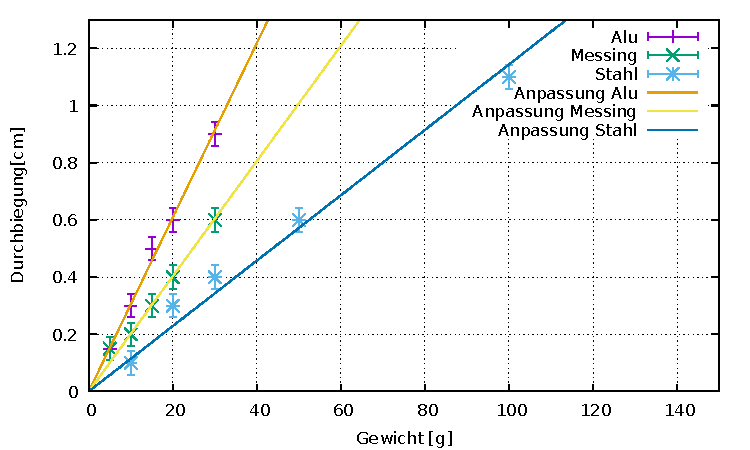
\includegraphics[width=1\textwidth]{res/Rund.pdf}
	\caption{Durchbiegung der Runden Stäbe in Abhängigkeit vom Gewicht.}
	\label{figdurchbiegungRund}
\end{figure}

\begin{figure}[h]
	\centering
	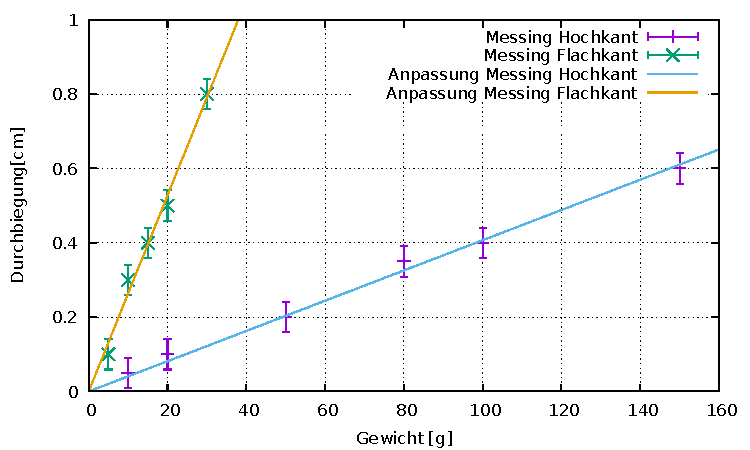
\includegraphics[width=1\textwidth]{res/Eckig.pdf}
	\caption{Durchbiegung des in zwei verschiedenen Ausrichtungen eingespannten Rechteckigen Stabes in Abhängigkeit vom Gewicht.}
	\label{fig:durchbiegungEckig}
\end{figure}


\begin{table}[h]
	\caption{Literaturwerte für das Elastizitätsmodul}
	\begin{tabular}{|c|c|}
		\hline
		& Elastizitätsmodul E $\left[\frac{GN}{m^2}\right]$\\
		\hline
		Aluminium & 70 \\
		\hline
		Eisen & 190 \\
		\hline
		Kupfer & 110 \\
		\hline
		Messing & 90 \\
		\hline
	\end{tabular}
\label{tab:ElaLit}
\end{table}
%Fitfunktion Unsicherheit der Fitfunktion Warum die von Gnuplot?